\subsection*{1.3}

\subsubsection*{الف}
زبان 
\[L = \{w \,|\, w \in \{0, 1\}^{*} \,and\, w = w^R\}\]
رشته‌هایی را شامل می‌شود که توالی آن‌ها با توالی معکوس آن‌ها برابر است. در عبارت دیگر، این زبان شامل رشته‌های پالیندروم است.

\subsubsection*{ب}
برای اینکه ماشین بتواند رشته‌های با طول زوج را بپذیرد، باید از حالت $q_1$ بدون دریافت ورودی به $q_2$ بتوانیم بریم. برای اینکار، می‌توانیم یک ترانزیشن $\epsilon, \epsilon \to \epsilon$ بین این دو حالت اضافه کنیم. با این کار، ماشین می‌تواند زبان $L$ را بپذیرد.

\subsection*{2.3}

\subsubsection*{الف}
برای این قسمت زبانی که داریم به شکل زیر است:
\[L = \{a^i b^j \,|\, i = j \,or\, i = 3j\}\]
برای نشان دادن این زبان با یک ماشین پشته‌ای، می‌توانیم یک گرامر مستقل از متن به شکل زیر تعریف کنیم:

\begin{align*}
	S &\to A | B \\
	A &\to aAb | \epsilon \\
	B &\to aaBbb | \epsilon \\
\end{align*}

\begin{center}
	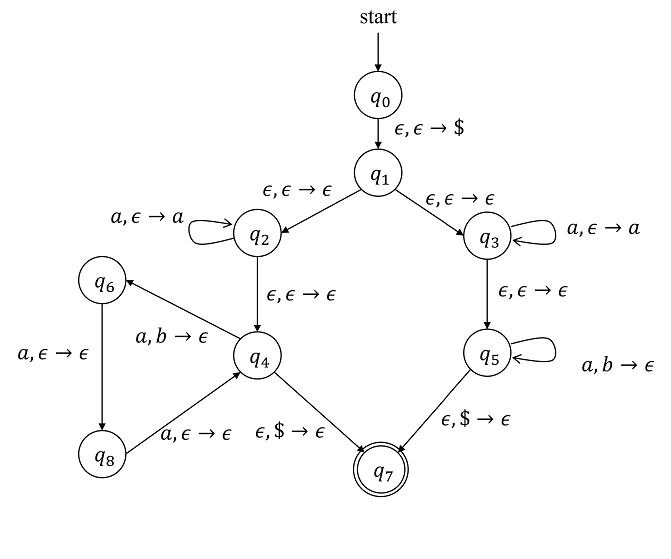
\includegraphics{image3}
\end{center}

\subsubsection*{ب}
زبان بعدی به شکل زیر است:
\[L = \{a^i b^j c^k \,|\, k \geq \min(i, j)\}\]
برای نشان دادن این زبان با یک ماشین پشته‌ای، می‌توانیم یک گرامر مستقل از متن به شکل زیر تعریف کنیم:

\begin{align*}
	S &\to AS | BS | T \\
	A &\to aAc | \epsilon \\
	B &\to bBc | \epsilon \\
	T &\to cT | \epsilon \\
\end{align*}

\begin{center}
	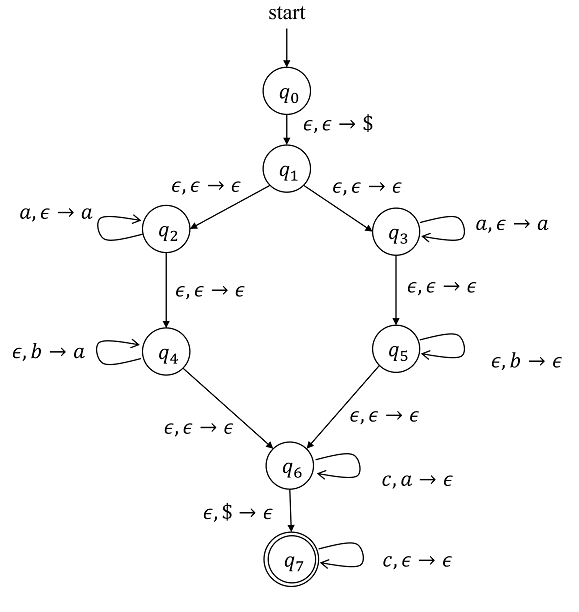
\includegraphics{image4}
\end{center}

\subsubsection*{ج}
زبان بعدی به شکل زیر است:
\[L = \{0^n 1^m \,|\, n \ne 2m + 1 \,and\, n,m > 0\}\]
برای نشان دادن این زبان با یک ماشین پشته‌ای، می‌توانیم یک گرامر مستقل از متن به شکل زیر تعریف کنیم:

\begin{align*}
	S &\to 0S1 | 00S11 | 0T1 \\
	T &\to 0T1 | \epsilon \\
\end{align*}

\begin{center}
	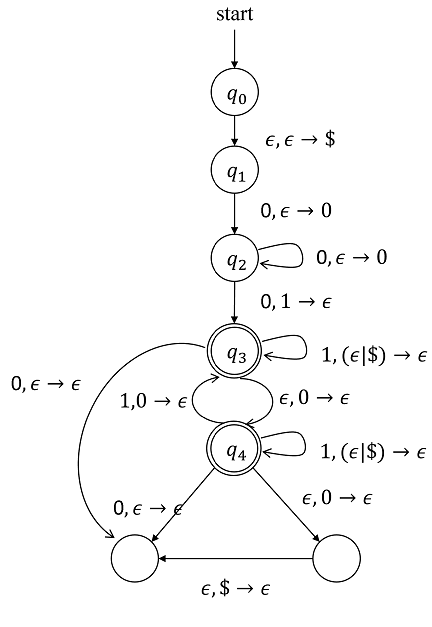
\includegraphics{image5}
\end{center}